\documentclass[tikz,border=10pt]{standalone}
\begin{document}
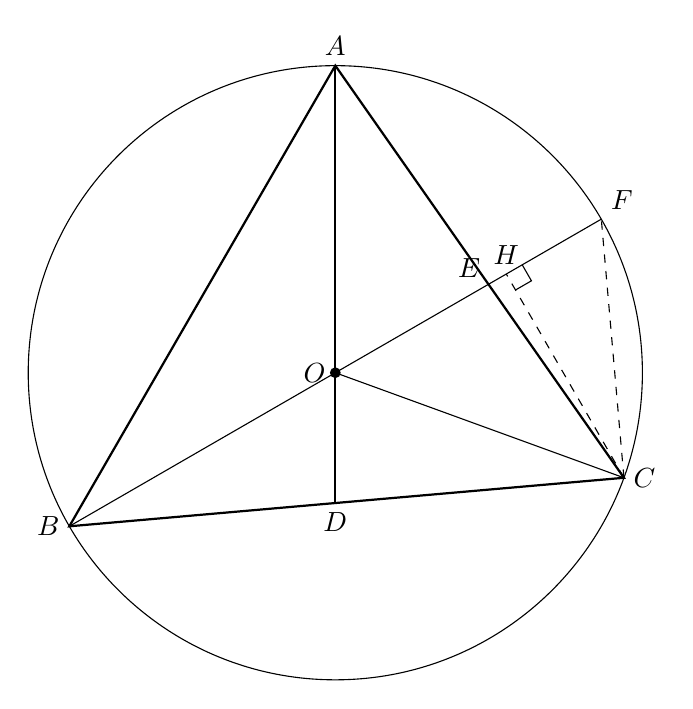
\begin{tikzpicture}[scale=1.3]
\coordinate (O) at (0,0);
\coordinate (A) at (0,3);
\coordinate (B) at (-2.598,-1.5);
\coordinate (C) at (2.819,-1.026);
\coordinate (D) at (0,-1.273);
\coordinate (F) at (2.598,1.5);
\coordinate (E) at (1.511,0.839);
\coordinate (H) at (1.670,0.964);

\draw (O) circle (3);

\draw[thick] (A) -- (B) -- (C) -- cycle;
\draw[thick] (A) -- (D);
\draw (B) -- (F);
\draw (O) -- (C);
\draw (O) -- (D);
\draw[dashed] (C) -- (H);
\draw[dashed] (C) -- (F);

% right angle mark at H
\draw (1.826,1.054) -- (1.916,0.898) -- (1.760,0.808);

\fill (O) circle (1.5pt);

\node[above] at (A) {$A$};
\node[left] at (B) {$B$};
\node[right] at (C) {$C$};
\node[below] at (D) {$D$};
\node[above right] at (F) {$F$};
\node[above left] at (E) {$E$};
\node[above] at (H) {$H$};
\node[left] at (O) {$O$};
\end{tikzpicture}
\end{document}
